
% --------------- 12 POINT FONT -------------------------------
\documentclass[12pt]{article}
% --------------- 10 POINT FONT FOR CAPTIONS ------------------
\usepackage[font=footnotesize]{caption}
% --------------- NY TIMES FONT -------------------------------
\usepackage{times}
% --------------- 1 INCH MARGINS ------------------------------
\usepackage[margin=1in]{geometry}
% --------------- LINE SPACING --------------------------------
\usepackage{setspace}
\singlespacing
%\doublespacing
% --------------- SMALL SECTION TITLES ------------------------
\usepackage[tiny,compact]{titlesec}
% --------------- PACKAGES ------------------------------------
\usepackage{bookmark}
\usepackage{algorithm}
\usepackage{algpseudocode}
\usepackage{amsfonts}
\usepackage{amsmath}
\usepackage{amssymb}
\usepackage{amsthm}
\usepackage{bm}
\usepackage{color}
\usepackage{comment}
\usepackage{float}
\usepackage{graphicx}
%\usepackage[hidelinks]{hyperref}
\usepackage{makecell}
\usepackage[caption=false,font=footnotesize,subrefformat=parens,labelformat=parens]{subfig}
\usepackage{wrapfig}
\usepackage{url}
\usepackage[table]{xcolor}
\graphicspath{{images/}}
\begin{document}
% --------------- TITLE AND NAME ------------------------------
\begin{center}
\textbf{Summary}\\
\end{center}

\noindent
Bardia Mojra\\
\today\\
Seminar on Continual Learning\\
Robotic Vision Lab\\
% --------------- CONTENT -------------------------------------
\begin{center}
A Simple Approach to Continual Learning By\\
Transferring Skill Parameters\\
\end{center}
\begin{center}
  {\small K.R. Zentner, Ryan Julian, Ujjwal Puri, Yulun Zhang, and Gaurav S. Sukhatme}\\
\end{center}

Learning robotic manipulation tasks from vision is challenging and requires
massive amount of data and hundreds of hours of training. In recent years,
physics-based simulators and Deep Reinforcement Learning (DRL) algorithms have
been widely
used to allow learning agents to explore the solution space and construct rich
function approximators or policy functions. In such end-to-end approaches,
researchers train a Deep Neural Network (DNN) with both visual input and
motor control output data provided at the same time but rather in short and
similar episodes. Nonetheless, the main issue with this approach is the fact
that it is still too computationally expensive to learn new skills from scratch or
to even retrain after transfer learning.\\

The authors introduce a novel and more efficient method for
continual learning of manipulation tasks by transferring skill parameters. They
show that representing past experiences only in form of skill policies,
methodical pretraining, and appropriately choosing when to
transfer those skill policies is a simple yet effective recipe for building a
continual learner in the context of robotic manipulation. New skill policies are
learned based on \textit{prior skills} or \textit{skill libraries} to enable
efficient acquisition and transfer of dynamic control policies. Similar to
\cite{hausman2018learning} and \cite{julian2018scaling}, they train reuseable
skill libraries in simulation to develop composable skill policies in form
of latent space parameter.

latent state representation of decomposed
skills for learning reuseable skill libraries based on decomposition.
    through  learned skills by transferring skill parameters directly.\\


\noindent
\textbf{Setting}\\
They define continual learning problem as iterated transfer learning for
multi-task reinforcement learning (MTRL) on a possibly-unbounded discrete space
of tasks \(\mathcal{T}\).
S a single continuous state space shared among all tasks T.
A a single continuous action space shared among all tasks T.
The MTRL problem is defined by \((\mathcal{T},~S,~A)\) and each task
\(\tau \in \mathcal{T}\) is an infinite-horizon Markov decision process (MDP)
defined as
\begin{equation}
\tau = \left(S, A, p_{\tau} (s,a,s'), r_{\tau} (s,a,s') \right).
\end{equation}
\noindent
Tasks are differentiated only by their reward functions \(r_{\tau}\) and
state transition dynamics \(p_{\tau}\). Thus, for simplicity they define
\begin{equation}
\tau = \left( r_{\tau}, p_{\tau}\right).
\end{equation}
\noindent
Importantly, the authors did not presume the robot has access to all tasks in
T at once or even a representative sample. The robot can only access one task at
a time. The time between task transitions is referred to as an 'epoch' with
each having a unique index. Tasks may reapear and when solving a "target task,"
the robot can only skill policies acquired while solving prior tasks M (the
'skill library"). Thus, they redefine the MTRL
\begin{equation}
\tau = \left(S, A, M_{i}, p_{\tau_{i}} (s,a,s'), r_{\tau_{i}} (s,a,s') \right),
\end{equation}
\noindent
where \(M_i\) represents the set manipulation skills the robot is initialized
with and \(i\) is the epoch number.


\noindent
\textbf{Simple Continual Learning with Skill Transfer}\\
\begin{figure}[h]
  \centering
  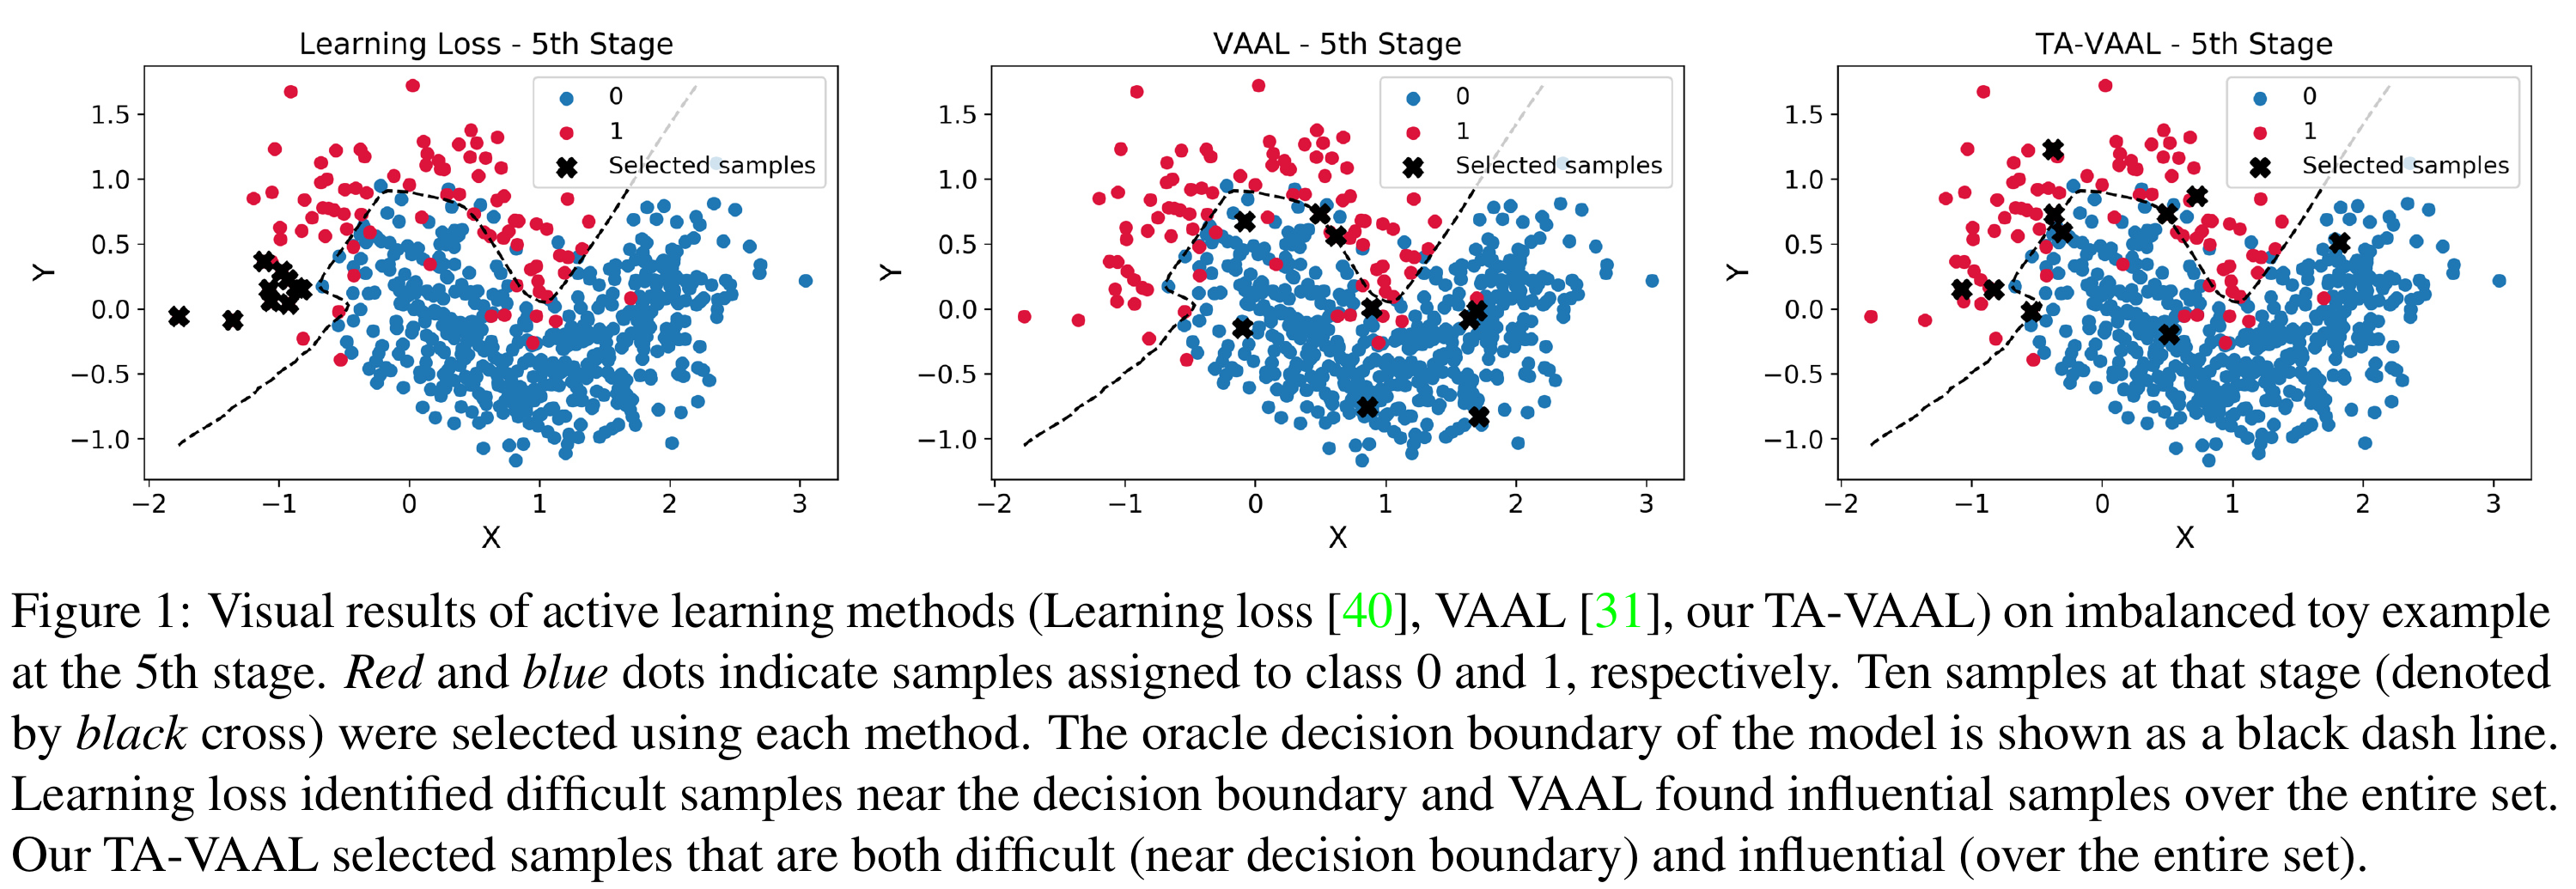
\includegraphics[width=1\textwidth]{/fig01.png}
  \caption{Algorithm 1}
\end{figure}




%\newpage
% Figure 2 depicts latent space variable projections onto $z_1 \times z_2$ phase plane.

% \begin{figure}[h]
%   \centering
%   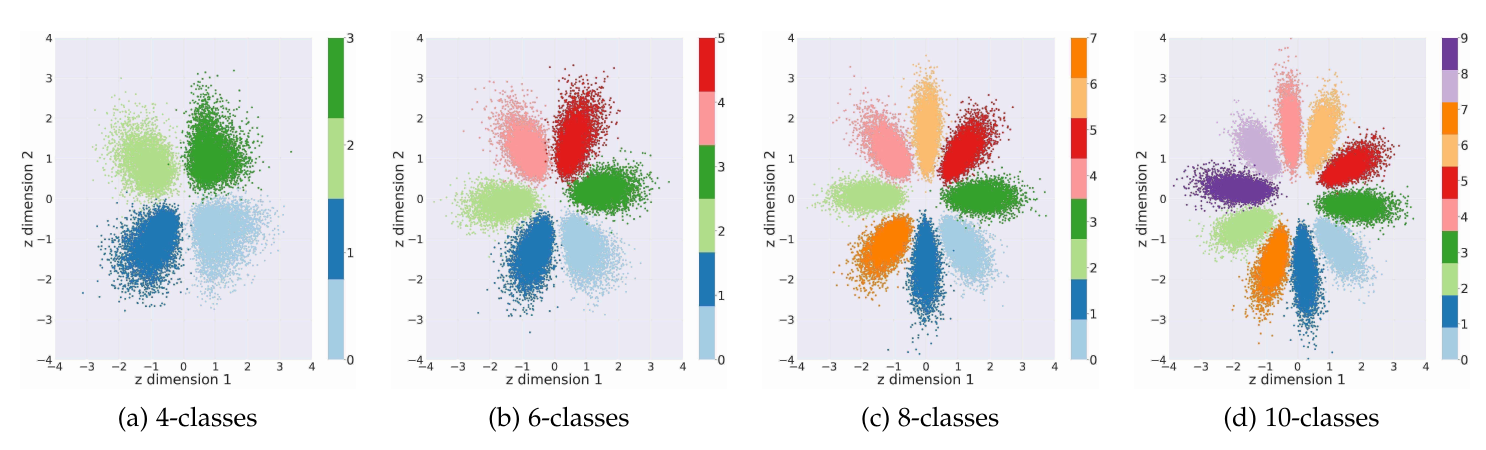
\includegraphics[width=.9\textwidth]{../z_phase.png}
%   \caption{2-D latent space visualization for continually learned MNIST.}
% \end{figure}


%Sets the bibliography style to UNSRT and import the
\newpage
\bibliography{ref}
\bibliographystyle{ieeetr}

\end{document}
